\graphicspath{{Images/}}

\section{LCSR for $D_{s}^{+}\to\eta^{(\prime)}$}

\subsection{Correlation Function}

LCSR starts with the correlation function Eq.\ref{eq:correlation_function}.

\begin{equation}
    \Pi_\mu(p, q)=i \int d^4 x e^{i q x}\left\langle \eta^{(\prime)}(p)\left|\mathrm{T}\left\{j_{\mu,1}(x), j_{2}(0)\right\}\right| 0\right\rangle
    \label{eq:correlation_function}
\end{equation}

In reference~\cite{JHEP1}, the currents entering the correlation function are defined as shown in Table~\ref{tab:Currents}.

\begin{table}[htbp]
    \centering
    \caption{Currents entering the correlation function\cite{JHEP1}.}
    \vspace{4mm}
    \begin{tabular}{c | c c}
        \hline \hline
        \textbf{Decay}                                                                  & \textbf{Interpolation current}                                                                           & \textbf{Weak current} \\
        \hline
        \multirow{2}{*}{$D_{s}^{+}\rightarrow\eta^{(\prime)}l^{+}\nu_{l}$}              &
        \multirow{2}{5cm}{~~~~$j_{2} = j_{D_s^{+}}^{\dagger}=m_c \bar{c} i \gamma_5 s$} &
        $j_{\mu,1} = V_\mu^{\left(\eta, \eta^{\prime}\right)}=\bar{s} \gamma_\mu c$                                                                                                                                        \\
                                                                                        &
                                                                                        & $\Tilde{j}_{\mu,1} = \Tilde{V}_\mu^{\left(\eta, \eta^{\prime}\right)}=\bar{s} \sigma_{\mu\nu} q^{\nu} c$                         \\
        \hline\hline
    \end{tabular}
    \label{tab:Currents}
\end{table}

The Feynman diagram corresponding to the formula is shown in fig.\ref{fig:feynman1}.

\begin{figure}[!hpt]\centering
    \rotatebox{90}{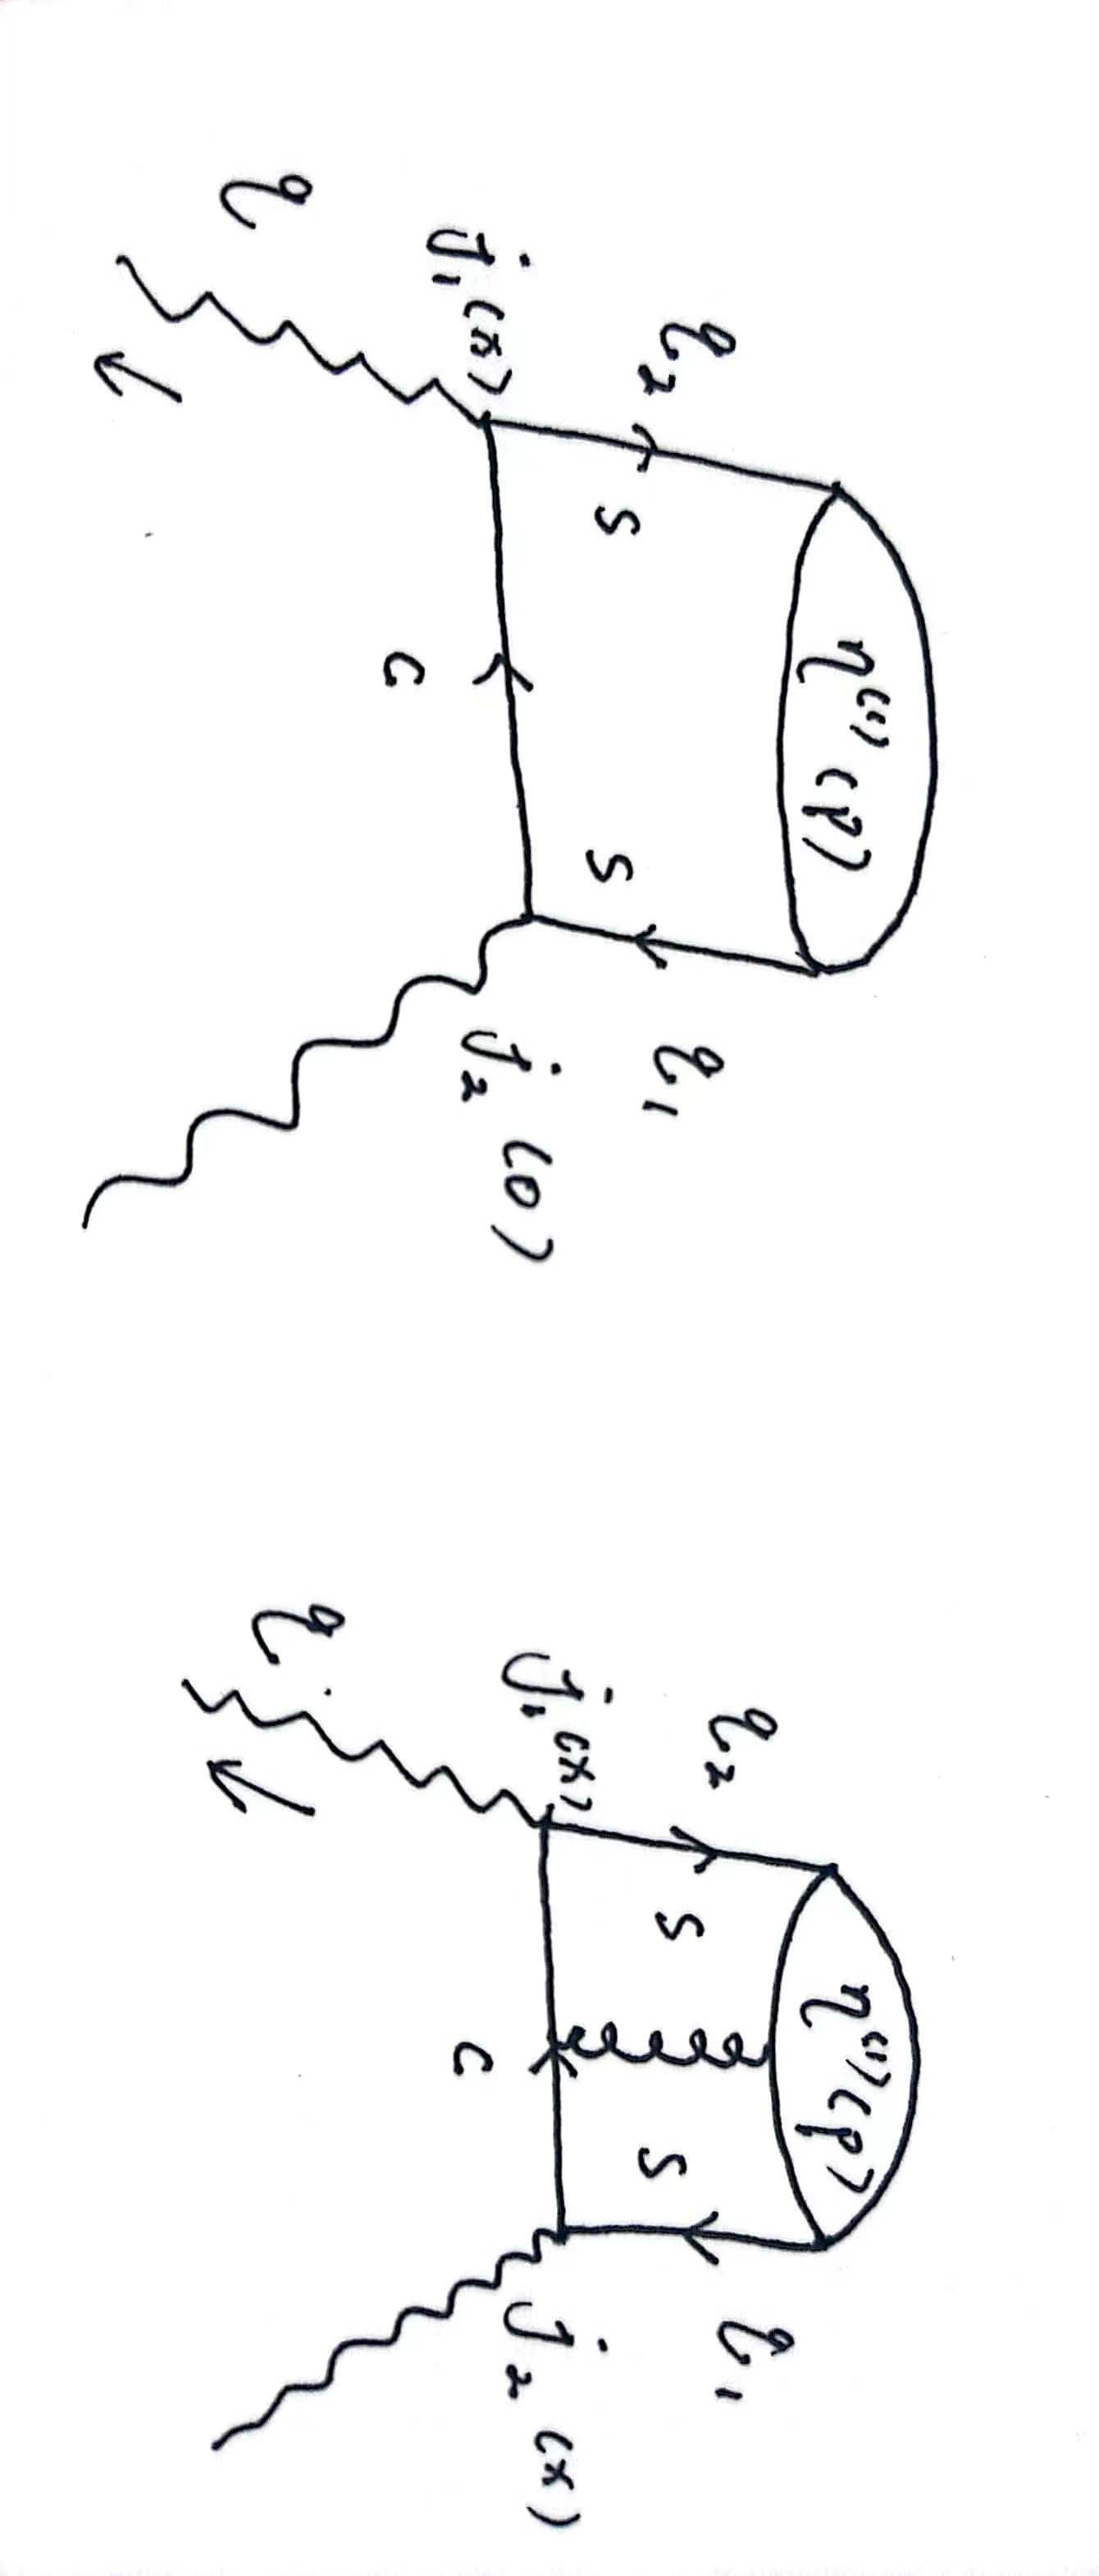
\includegraphics[width=0.3\textwidth]{image/feynman.jpg}}
    \caption{Diagrams corresponding to the leading-order terms in the hard-scattering amplitudes
        involving the two-particle (left) and three-particle (right)}
    \label{fig:feynman1}
\end{figure}

It has been showen by Källén and Lehmann~\cite{Kallen1952, Lehmann1954} quite a long time ago that the two-point correlation functions obey dispersion relation:

\begin{equation}
    \Pi_\mu(p, q)= \int_{0}^{\infty} dt\, \rho_{\mu}(t)\frac{1}{t-(p+q)^{2}-i\epsilon}
\end{equation}

For $(p+q)^{2}>0$, we have

\begin{equation}
    \begin{array}{rl}
        \Pi_\mu(p, q) & = \mathcal{P} \int_{0}^{\infty} dt\, \rho_{\mu}(t)\frac{1}{t-(p+q)^{2}} + i\pi\rho_{\mu}((p+q)^{2}) \\
                      & = \mathrm{Re}\Pi_\mu(p, q) + \mathrm{Im}\Pi_\mu(p, q)
    \end{array}
    \label{eq:dispersion_relation_real}
\end{equation}

Clearly, $\mathrm{Im}\Pi_\mu(p, q)$ has a corresponding relationship with $\pi\rho_{\mu}((p+q)^{2})$, the spectral function density $\rho_{\mu}((p+q)^{2})$ is a scalar function of the Lorentz invariant $(p+q)^{2}$.

\begin{equation}
    \rho_{\mu}(t) = \frac{1}{\pi} \mathrm{Im}\Pi_\mu(t) \equiv \sum_{\Gamma}^{} \langle \eta^{(\prime)}|j_{\mu,1}|\Gamma\rangle \langle \Gamma|j_{2}|0\rangle (2 \pi)^4 \delta^{(4)}\left(q-p_{\Gamma}\right)
\end{equation}

Given the definition of $\mathrm{Im}\Pi_\mu(t)$, naturally, we have

\begin{equation}
    \Pi_\mu(p, q)= \frac{1}{\pi} \int_{0}^{\infty} dt\, \frac{\mathrm{Im}\Pi_\mu(t)}{t-(p+q)^{2}-i\epsilon}
    \label{eq:dispersion_relation}
\end{equation}


\subsection{Hadron Representation}
After inserting a complete set of hadronic states, specifically $|D_{s}^{+}(p+q)\rangle$, we have $(p+q)^{2} \geq m_{Ds}$ in the physical region.
\begin{equation}
    \begin{aligned}
        \Pi_\mu(p, q)^{hadron} & = i \int d^4 x e^{i q x}\left\langle \eta^{(\prime)}(p)\left|\mathrm{T}\left\{j_{1}(x), j_{2}(0)\right\}\right| 0\right\rangle + \frac{1}{\pi}  \int_{s_0}^{\infty} dt\, \frac{\mathrm{Im}\Pi_\mu^{hadron}(t)}{t-(p+q)^{2}-i\epsilon} \\
                               & = \frac{-i m_{D_s}^2 f_{D_s}[2 f_{D_{(s)} \eta^{(\prime)}}^{+}\left(q^2\right) p_\mu+\left(f_{D_{(s)} \eta^{(\prime)}}^{+}\left(q^2\right)+f_{D_{(s)} \eta^{(\prime)}}^{-}\left(q^2\right)\right)q_\mu]}{(m_c+m_s)[m^{2}_{D_{s}^{+}} - (p+q)^{2}]} \\
                               & \quad + \frac{1}{\pi} \int_{s_0}^{\infty} dt\, \frac{\mathrm{Im}\Pi_{+}^{hadron}(t,q^{2})p_{\mu} + \mathrm{Im}\Pi_{-}^{hadron}(t,q^{2})q_{\mu}}{t-(p+q)^{2}-i\epsilon}
    \end{aligned}
    \label{eq:hadron_rep}
\end{equation}
where $f_{D_{(s)} \eta^{(\prime)}}^{+}$ and $f_{D_{(s)} \eta^{(\prime)}}^{-}$ are the form factors defined as Eq.\ref{eq:form_factor}:
\begin{equation}
    \begin{aligned}
         & \left\langle \eta^{(\prime)}|j_{\mu,1}|D_{s}^{+}(p+q)\right\rangle=2 f_{D_{(s)} \eta^{(\prime)}}^{+}\left(q^2\right) p_\mu+\left(f_{D_{(s)} \eta^{(\prime)}}^{+}\left(q^2\right)+f_{D_{(s)} \eta^{(\prime)}}^{-}\left(q^2\right)\right) q_\mu,
    \end{aligned}
    \label{eq:form_factor}
\end{equation}

\subsection{Quark Representation}
Computed in the perturbative theory with the help of OPE technique at the deep Euclidean region $(p^{2}, q^{2} = -Q^{2} \ll 0)$, we have:

\begin{equation}
    \begin{aligned}
        \Pi_\mu(p, q)^{OPE} &= i \int d^4 x e^{i q x}\left\langle \eta^{(\prime)}(p)\left|\mathrm{T}\left\{j_{\mu,1}(x), j_{2}(0)\right\}\right| 0\right\rangle    \\
        &= i \int d^4 x e^{i q x}\left\langle \eta^{(\prime)}(p)\left|\mathrm{T}\left\{\bar{s}(x) \gamma_\mu c(x), \bar{c}(0) i \gamma_5 s(0)\right\}\right| 0\right\rangle 
    \end{aligned}
    \label{eq:quark_rep}
\end{equation}














